\subsection{Verwendete Komponenten}
\label{kap:McpExecutorVerwendeteKomponenten}
Für eine Einheit werden verschiedene Hardware-Komponenten verwendet, deren Wahl vor allem hinsichtlich des Kostenaufwandes erfolgte. Auch die Bauteilgröße ist ein entscheidender Faktor, da die Einheiten möglichst nicht störend sein sollen.

\begin{itemize}
	\item \textbf{Mcp2515}
	
	Der Mcp2515 beschreibt an sich den Chip, welcher auf der, in Abbildung \ref{fig:Mcp2515} dargestellten, Platine verbaut ist. Dieser Name wird jedoch für den gesamten Chip verwendet.
	\newline
	Die Funktion des Mcp2515 besteht darin Daten über die Schnittstelle SPI zu empfangen und über einen CAN-Bus zu versendet. Die Steuerung des Chips (z.B. Beschreiben eines Sende-Buffers) erfolgt dabei mit entsprechenden Kommandos über SPI. Das Konvertieren in L-, H-Pegel erfolgt komplett automatisch.
	
	\begin{figure}[H]
		\centering
		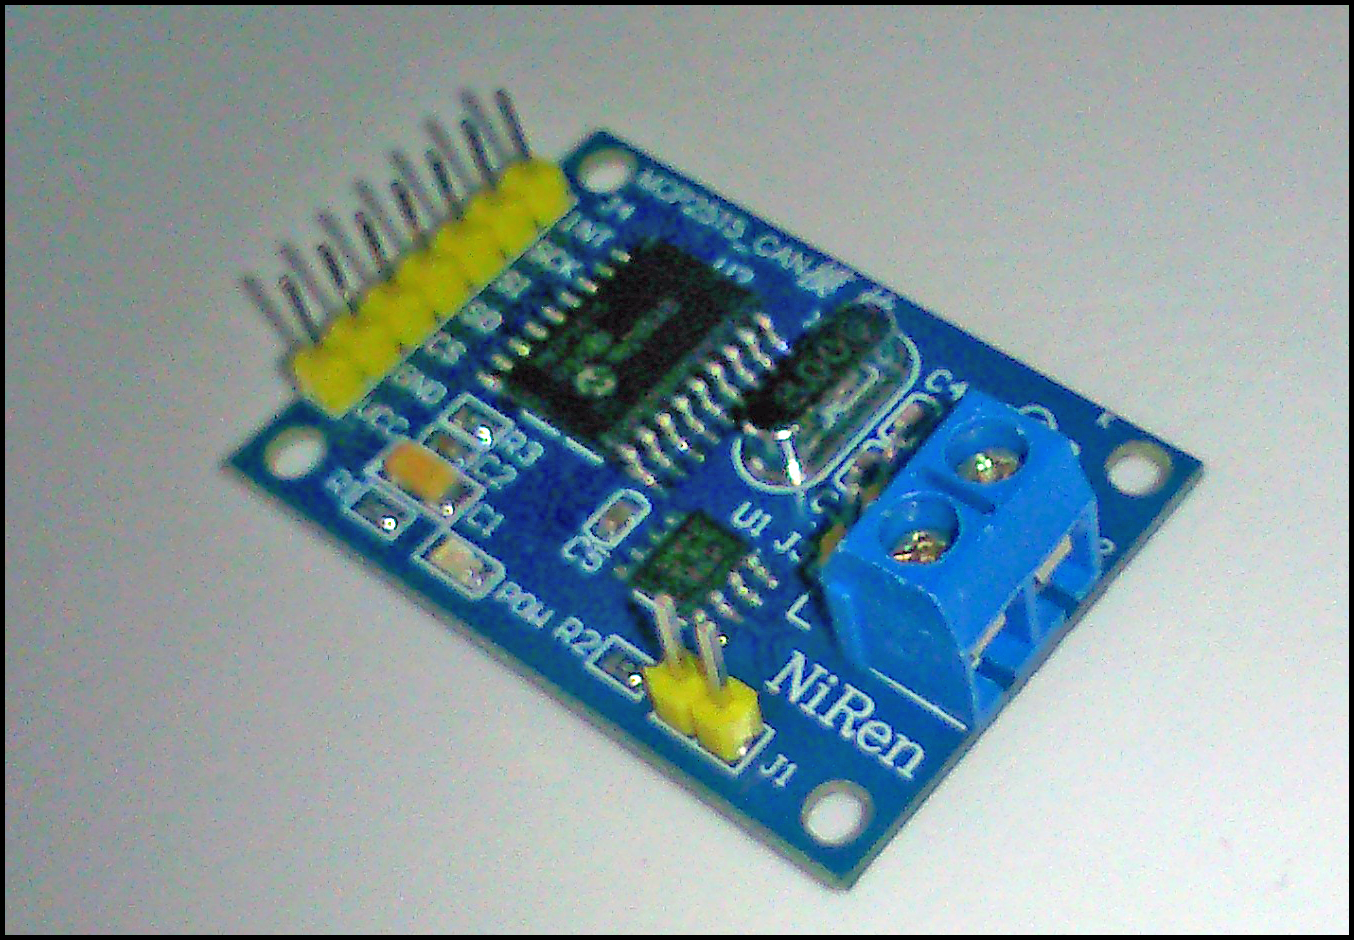
\includegraphics[width=0.4\linewidth]{Bilder/Mcp2515}
		\caption[Mcp2515]{Mcp2515}
		\label{fig:Mcp2515}
	\end{figure}
	
	\item \textbf{Adxl345}
	
	Bei dem Adxl345 handelt es sich um einen 3-Achsen Beschleunigungssensor (s. Abbildung \ref{fig:Adxl345}), dessen Messwerte über SPI in verschiedenen Genauigkeiten ausgelesen werden können.
	Der Chip besitzt eine äußerst geringe Leistungsaufnahme und ist kompatk in seiner Bauform.
		
	\begin{figure}[H]
		\centering
		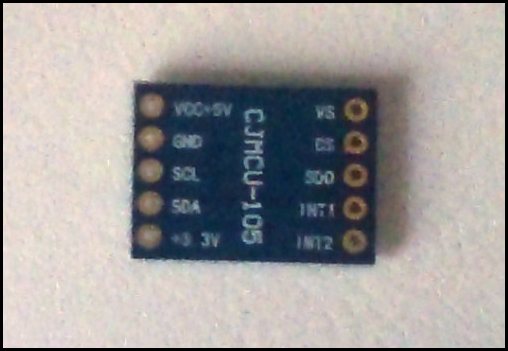
\includegraphics[width=0.4\linewidth]{Bilder/Adxl345}
		\caption[Adxl345]{Adxl345}
		\label{fig:Adxl345}
	\end{figure}
	
	\item \textbf{Atmega328}
	
	Der Microcontroller Atmega328 ist u.A. in dem Arduino-Board verbaut. Es ist ein kostenfünstiger Allrounder, welcher hauptsächlich wegen seiner großen Verbreitung gewählt wurde.
	Der Chip (s. Abbildung \ref{fig:Atmega328}) besitzt eine SPI-Schnittstelle und diverse I/O's, weshalb die Projektanforderungen vollständig erfüllt werden.
	\newline
	Es exisiteren zwei verschiedene Versionen des MCU's, von denen die Atmega328-P Variante für eine geringe Leistungsaufnahme konzipiert ist. 
	
	\begin{figure}[H]
		\centering
		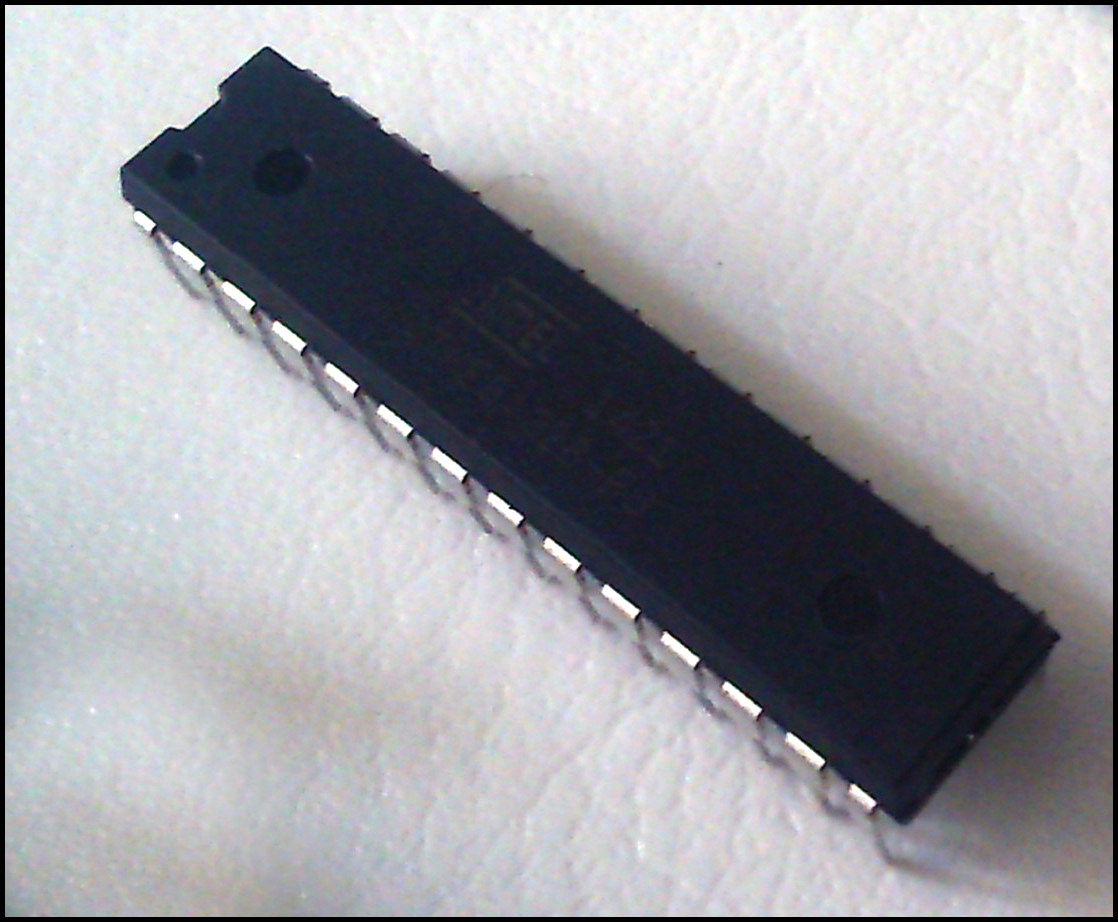
\includegraphics[width=0.4\linewidth]{Bilder/Atmega328}
		\caption[Atmega328]{Atmega328}
		\label{fig:Atmega328}
	\end{figure}
	
	\item \textbf{Oscillator und Kondensator}
	
	Der Atmega328 benötigt einen externen Taktgeber, welcher mit einem 16Mhz Quarz und entsprechenden Kondensatoren gewählt wird (s. Abbildung \ref{fig:Oscillator}).
	
	\begin{figure}[H]
		\centering
		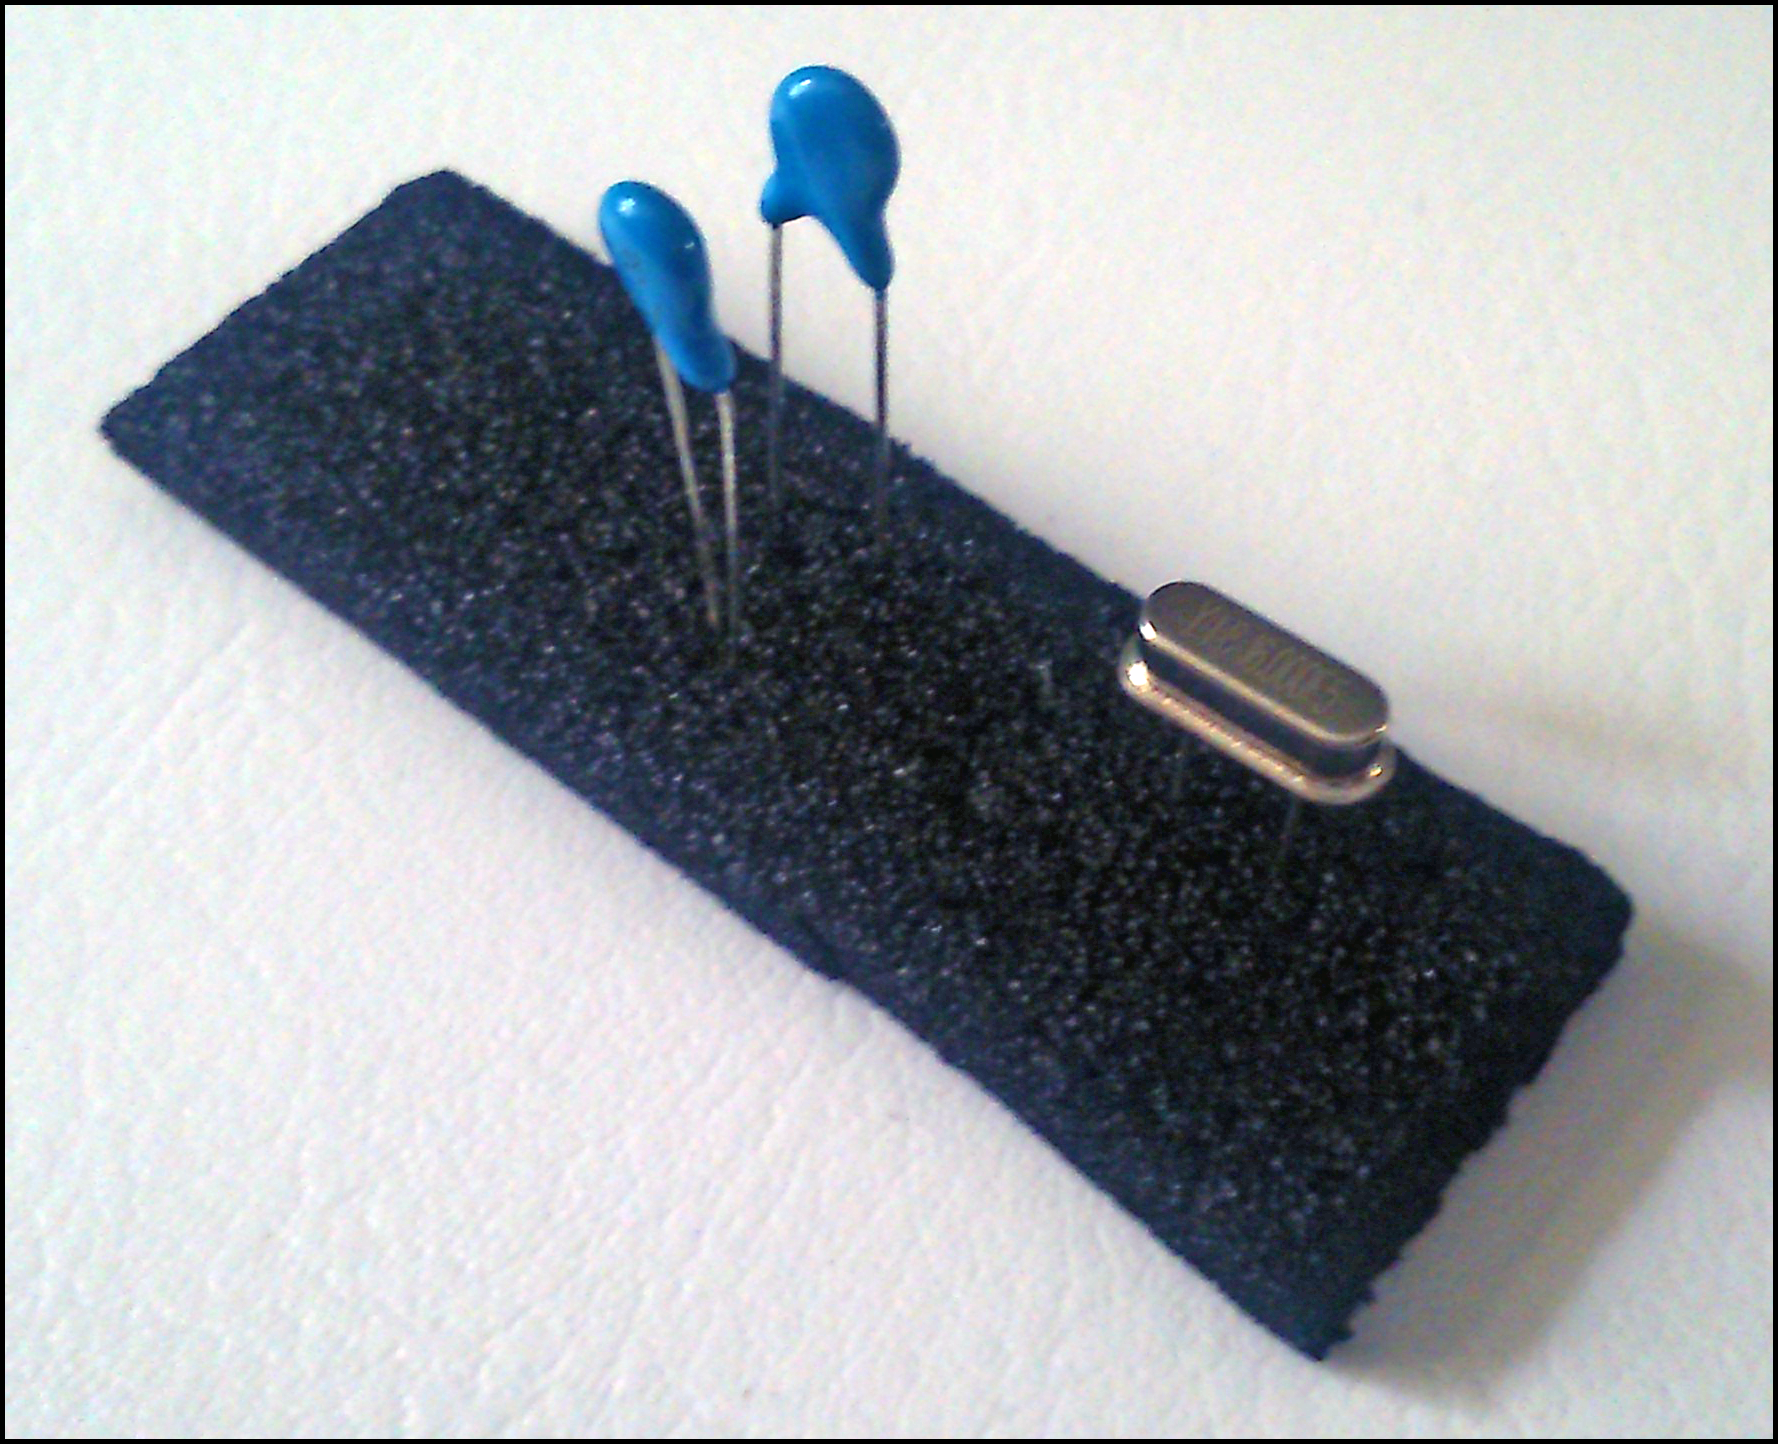
\includegraphics[width=0.4\linewidth]{Bilder/Oscillator}
		\caption[Oscillator]{Oscillator}
		\label{fig:Oscillator}
	\end{figure}
		
\end{itemize}